\documentclass[aspectratio=169]{beamer}

\mode<presentation>
{
  \usetheme{default}
  \usecolortheme{default}
  \usefonttheme{default}
  \setbeamertemplate{navigation symbols}{}
  \setbeamertemplate{caption}[numbered]
  \setbeamertemplate{footline}[frame number]  % or "page number"
  \setbeamercolor{frametitle}{fg=white}
  \setbeamercolor{footline}{fg=black}
} 

\usepackage[english]{babel}
\usepackage[utf8x]{inputenc}
\usepackage{tikz}
\usepackage{courier}
\usepackage{array}
\usepackage{bold-extra}
\usepackage{minted}
\usepackage[thicklines]{cancel}

\xdefinecolor{dianablue}{rgb}{0.18,0.24,0.31}
\xdefinecolor{darkblue}{rgb}{0.1,0.1,0.7}
\xdefinecolor{darkgreen}{rgb}{0,0.5,0}
\xdefinecolor{darkgrey}{rgb}{0.35,0.35,0.35}
\xdefinecolor{darkorange}{rgb}{0.8,0.5,0}
\xdefinecolor{darkred}{rgb}{0.7,0,0}
\definecolor{darkgreen}{rgb}{0,0.6,0}
\definecolor{mauve}{rgb}{0.58,0,0.82}

\title[2017-10-25-aps-nuclear]{Bridging the Particle Physics and Big Data Worlds}
\author{Jim Pivarski}
\institute{Princeton University -- DIANA-HEP}
\date{October 25, 2017}

\begin{document}

\logo{\pgfputat{\pgfxy(0.11, 7.4)}{\pgfbox[right,base]{\tikz{\filldraw[fill=dianablue, draw=none] (0 cm, 0 cm) rectangle (50 cm, 1 cm);}\mbox{\hspace{-8 cm}
\includegraphics[height=1 cm]{princeton-logo-long.png}
\includegraphics[height=1 cm]{diana-hep-logo-long.png}}}}}

\begin{frame}
  \titlepage
\end{frame}

\logo{\pgfputat{\pgfxy(0.11, 7.4)}{\pgfbox[right,base]{\tikz{\filldraw[fill=dianablue, draw=none] (0 cm, 0 cm) rectangle (50 cm, 1 cm);}\mbox{\hspace{-8 cm}
\includegraphics[height=1 cm]{princeton-logo.png}
\includegraphics[height=1 cm]{diana-hep-logo.png}}}}}

% Uncomment these lines for an automatically generated outline.
%\begin{frame}{Outline}
%  \tableofcontents
%\end{frame}

%%%%%%%%%%%%%%%%%%%%%%%%%%%%%%%%%%%%%%%%%%%%%%%%%%%%%%%

%%%% START

%% \begin{frame}{Particle physics: the original Big Data}
%% \vspace{0.5 cm}

%% \large For decades, our computing needs were unique:

%% \vspace{0.1 cm}
%% \begin{itemize}
%% \item large datasets \hfill \begin{minipage}{0.7\linewidth}(too big for one computer: a moving definition!),\end{minipage}
%% \item complex structure \hfill \begin{minipage}{0.7\linewidth}(nested data, web of relationships within each event),\end{minipage}
%% \item has to be reduced \hfill \begin{minipage}{0.7\linewidth}(aggregated, by histogramming, usually)\end{minipage}
%% \item to be modeled \hfill \begin{minipage}{0.7\linewidth}(fitting to extract physics results).\end{minipage}
%% \end{itemize}

%% \vspace{0.5 cm}
%% \uncover<2->{\textcolor{darkblue}{\large Today these criteria apply equally, or more so, to ``web scale data.''}}
%% \end{frame}

%% \begin{frame}{{200~PB is a lot of data}\only<2>{, but for Amazon, it's two trucks}}
%% \vspace{0.35 cm}
%% 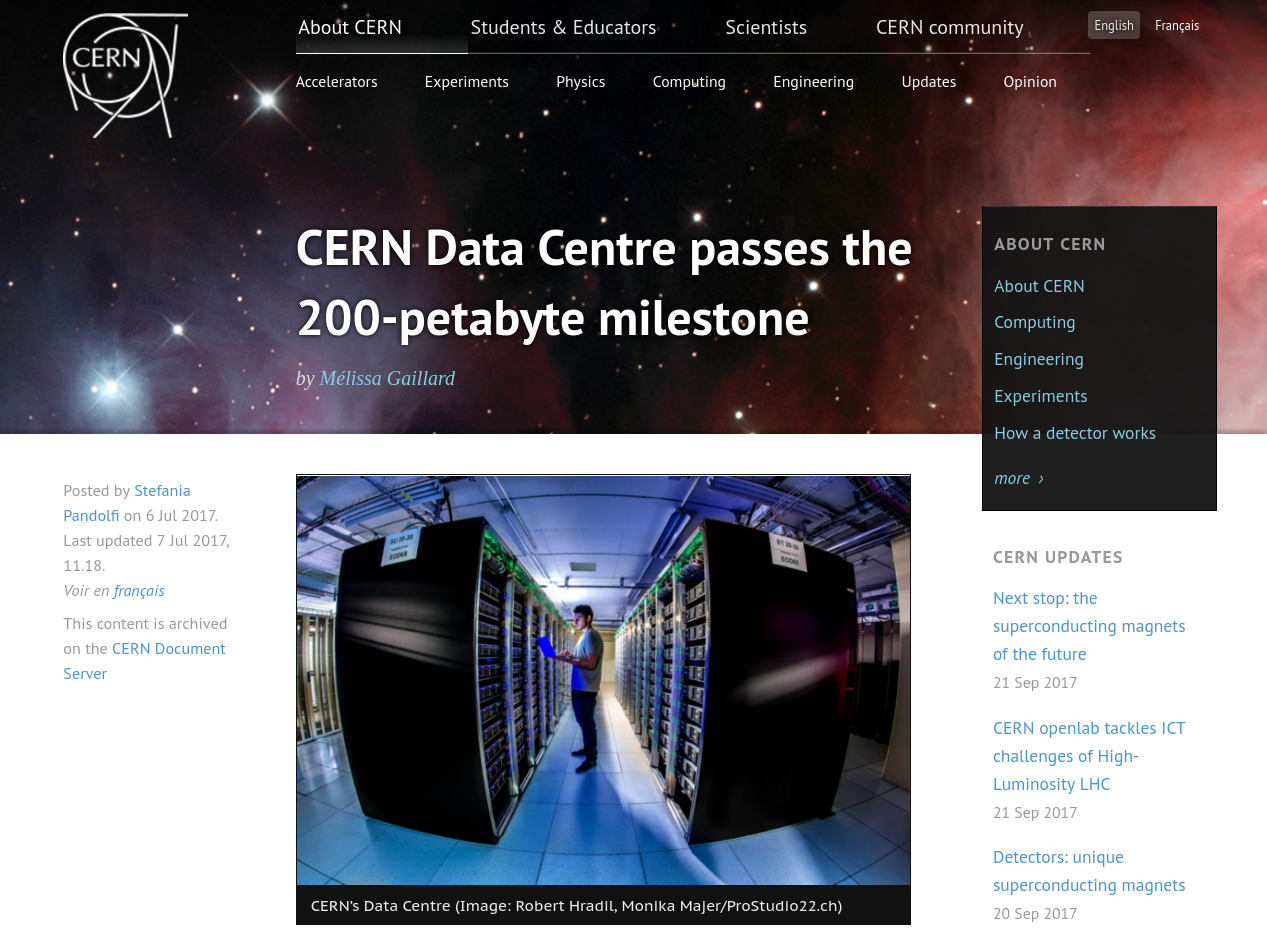
\includegraphics[width=0.73\linewidth]{cern-200pb.png}

%% \vspace{-4.8 cm}
%% \uncover<2->{\mbox{ } \hfill 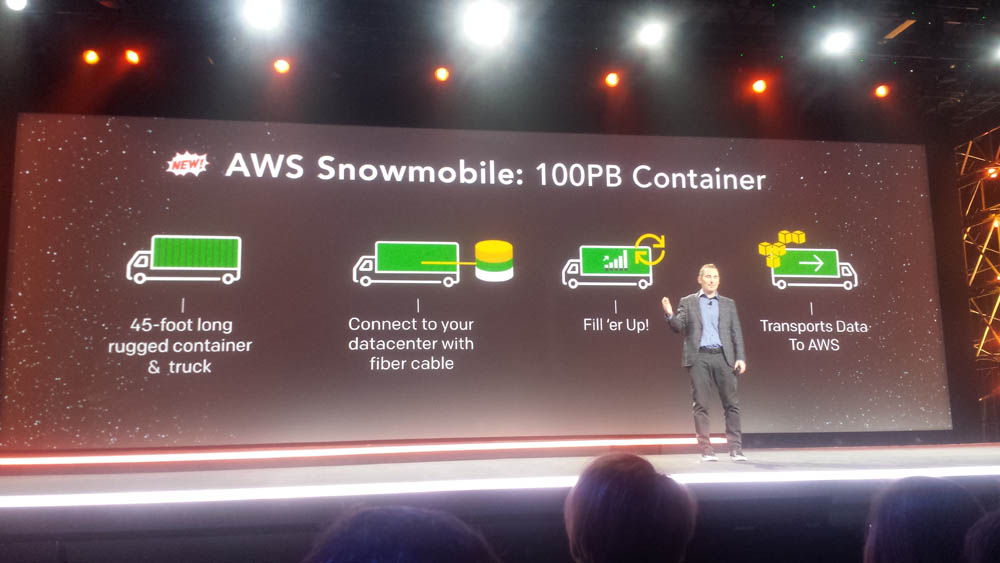
\includegraphics[width=0.7\linewidth]{aws-snowmobile.jpg}\hspace{-1 cm}}
%% \end{frame}

%% \begin{frame}{Also a much larger community}
%% \vspace{0.35 cm}
%% \textcolor{darkblue}{Rate of web searches for ``ROOT TTree'' vs.\ ``Spark DataFrame'' (Google Trends):}

%% 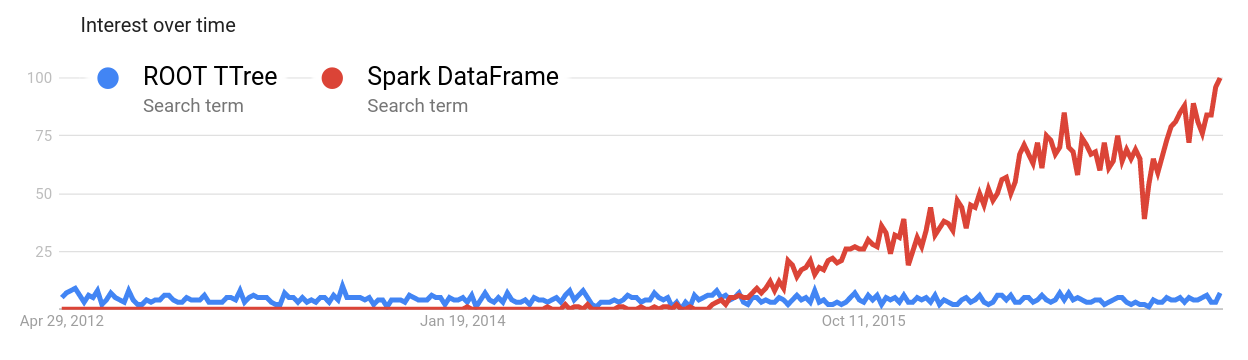
\includegraphics[width=\linewidth]{root-spark-google-trends.png}

%% \vfill
%% \begin{uncoverenv}<2->
%% \textcolor{darkblue}{Similarly for question-and-answer sites:}
%% \begin{itemize}
%% \item RootTalk: 14,399 threads in 1997--2012 (15 years)
%% \item StackOverflow questions tagged {\tt \small \#spark}: 26,155 in the 3.3 years the tag has existed. (Not counting CrossValidated, Spark Developer and User mailing lists\ldots)
%% \end{itemize}
%% \end{uncoverenv}

%% \vfill
%% \uncover<3>{\textcolor{darkorange}{\bf More users to talk to; more developers adding features/fixing bugs.}}
%% \end{frame}

%% \begin{frame}{Particle physics is a special case}
%% \vspace{-0.5 cm}
%% \begin{columns}[t]
%% \column{0.5\linewidth}
%% \begin{center}
%% \underline{\Large Particle physics}
%% \end{center}

%% \begin{itemize}
%% \item Events (modulo cosmics vetos or time-dependent calibrations) may be processed in isolation; embarrassingly parallel.

%% \item<2-> Once collected, physics datasets are immutable (with revisions).

%% \item<3-> Often fitting a model with a small number of parameters.

%% \end{itemize}

%% \column{0.5\linewidth}
%% \begin{center}
%% \underline{\Large Big Data}
%% \end{center}

%% \begin{itemize}
%% \item All-to-all problems are common, such as matching a customer's purchases with all other purchases to make a recommendation.

%% \item<2-> Transactions accumulate in the database during analysis.

%% \item<3-> Modeling human behavior, more interested in predictions than description, so models may have thousands of free parameters.

%% \end{itemize}

%% \end{columns}
%% \end{frame}

%% \begin{frame}{Our software is largely isolated from these developments}
%% \vspace{0.17 cm}
%% 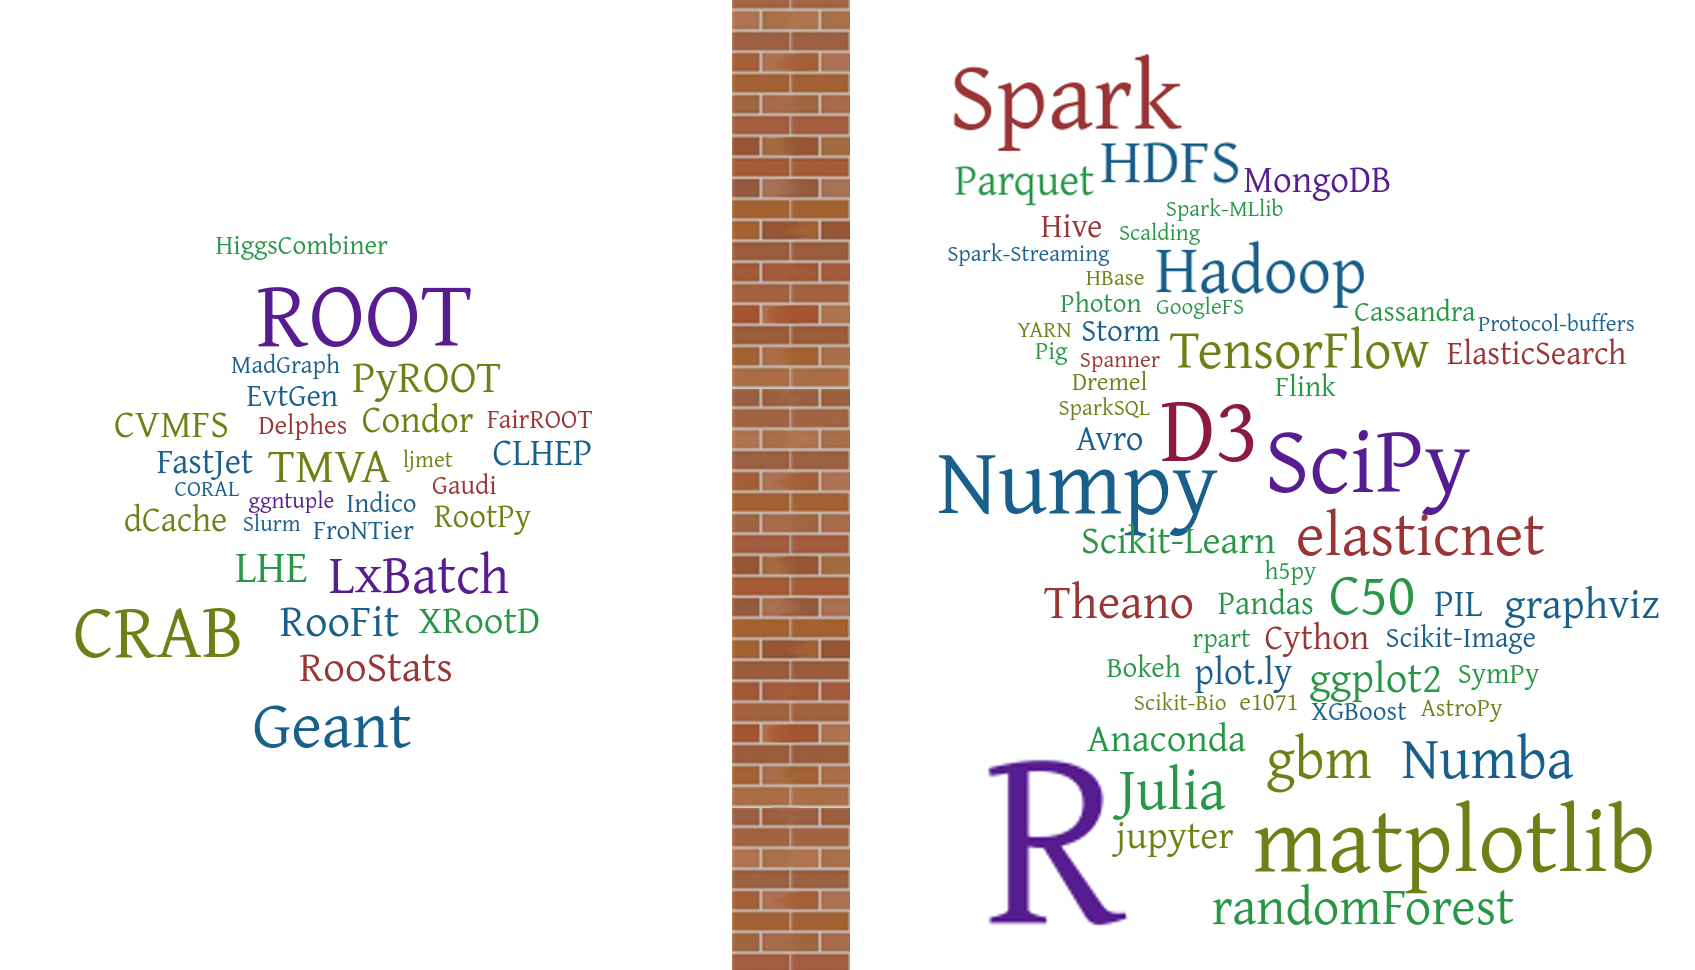
\includegraphics[width=\linewidth]{separation-2.png}
%% \end{frame}

%% \begin{frame}{Who am I?}
%% \vspace{0.5 cm}
%% \begin{columns}[t]
%% \column{0.4\linewidth}
%% \begin{columns}
%% \column{0.4\linewidth}
%% Jim Pivarski
%% \column{0.25\linewidth}
%% \hspace{-1.3 cm}
\includegraphics[width=\linewidth]{jim_pivarski.png}
%% \end{columns}

%% \begin{itemize}
%% \item 5 years CLEO (9 GeV $e^+e^-$)
%% \item 5 years CMS (7 TeV $pp$)
%% \item \only<1>{5 years Open Data Group}\only<2->{\mbox{\textcolor{darkblue}{5 years Open Data Group \hspace{0.9 cm}$\longrightarrow$\hspace{-3 cm}}}}
%% \item 2 years Project DIANA-HEP
%% \end{itemize}

%% \column{0.4\linewidth}
%% \uncover<2->{\textcolor{darkblue}{
%% hyperspectral imagery \\
%% automobile traffic \\
%% network security \\
%% Twitter sentiment \\
%% Google n-grams \\
%% DNA sequence analysis \\
%% credit card fraud detection
%% }}

%% \uncover<2->{\Large\textcolor{darkblue}{ and ``Big Data'' tools}}
%% \end{columns}

%% \vspace{0.5 cm}
%% \begin{center}
%% \uncover<3>{\textcolor{violet}{\bf My goal within DIANA-HEP is to make it easier for physicists to use Big Data tools in their analyses, particularly for interactive, exploratory analysis.}}
%% \end{center}
%% \end{frame}

%% \begin{frame}{}
%% \vspace{-0.22 cm}
%% \begin{center}
%% \only<1>{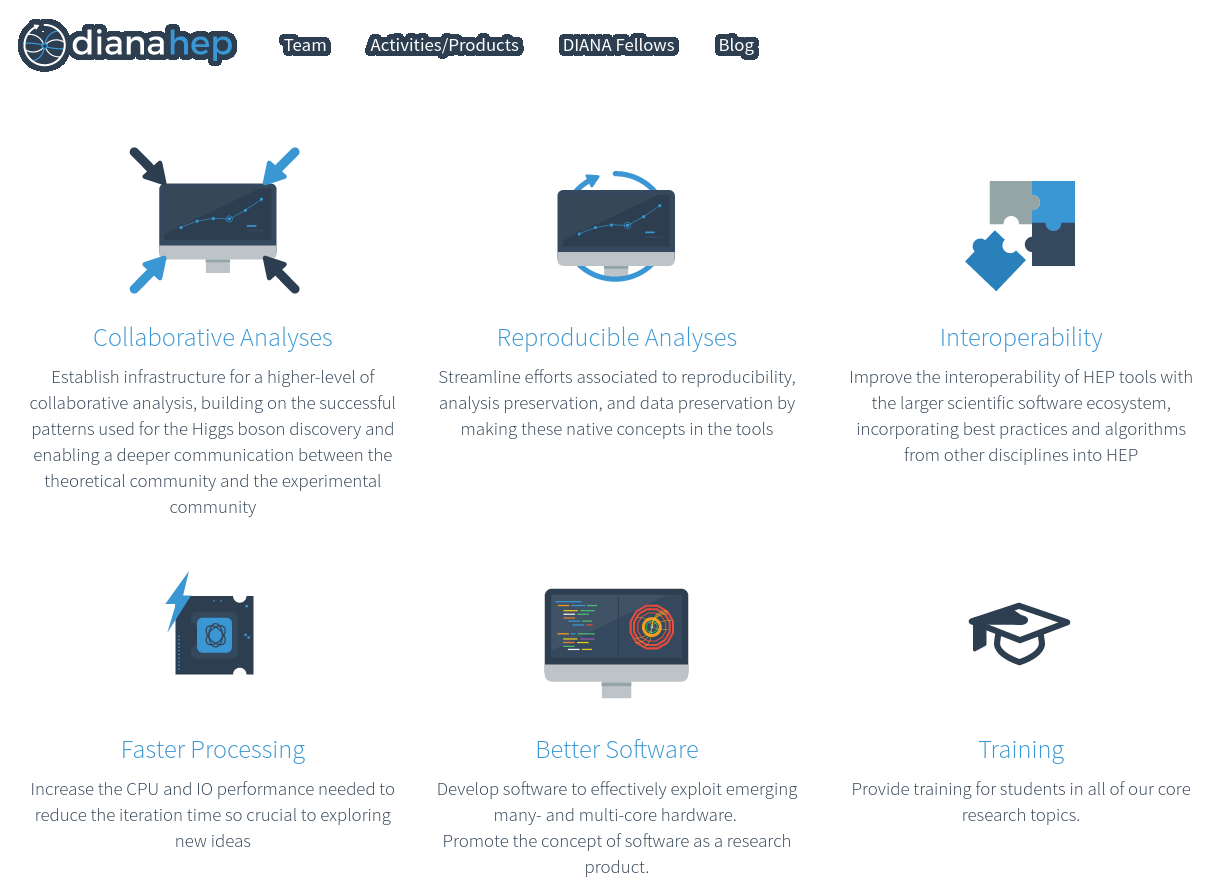
\includegraphics[width=0.88\linewidth]{diana-hep.png}}
%% \only<2>{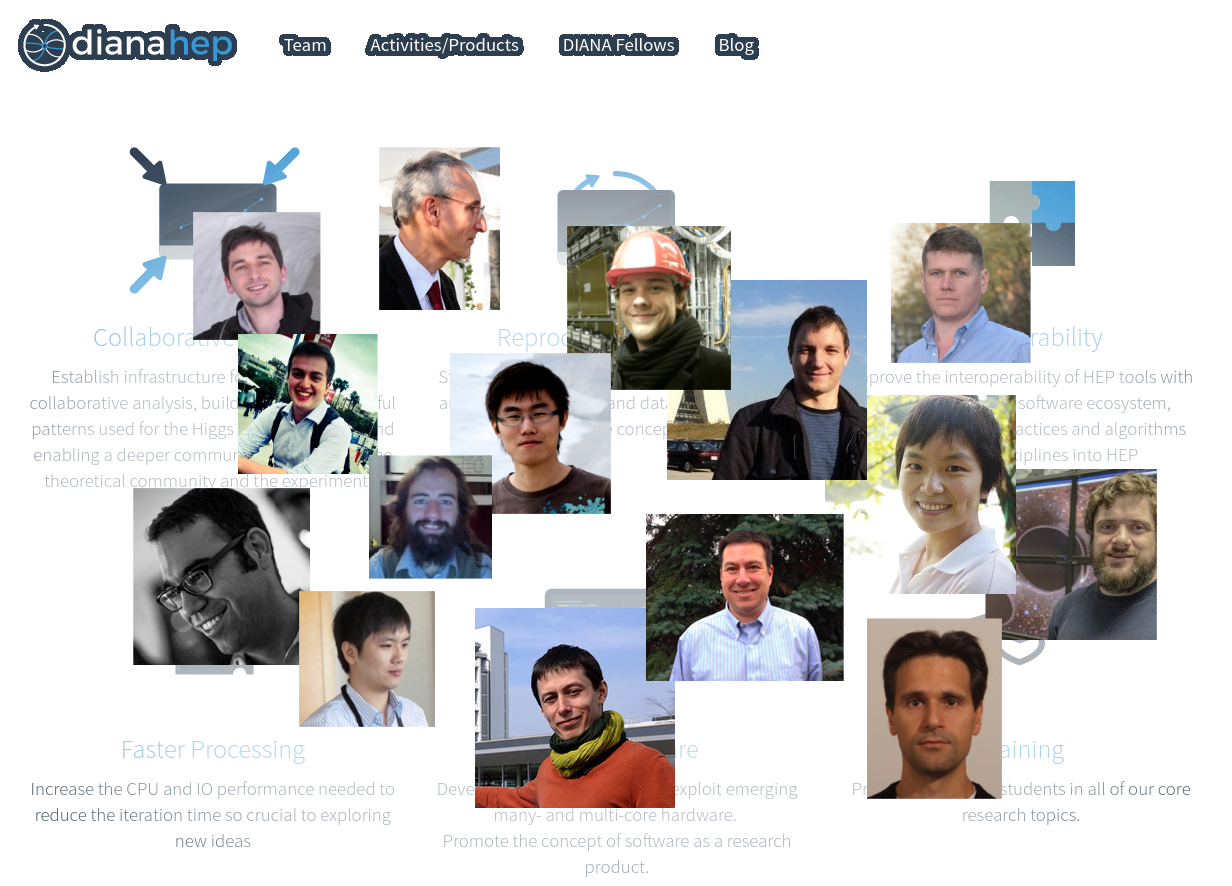
\includegraphics[width=0.88\linewidth]{diana-hep2.png}}
%% \end{center}
%% \end{frame}

%% \begin{frame}{Three types of physics software}
%% \vspace{0.25 cm}
%% \begin{columns}[t]
%% \column{0.33\linewidth}
%% \textcolor{darkblue}{\underline{Type I:}} Physics software that serves {\it the same function} as software in the Big Data community.

%% \begin{uncoverenv}<2->
%% \begin{center}
%% 
\includegraphics[height=1.5 cm]{stamp_replace.png}
%% \end{center}

%% Big Data community has better resources for
%% \begin{itemize}
%% \item maintaining code
%% \item catching bugs
%% \item revising bad designs.
%% \end{itemize}
%% \end{uncoverenv}

%% \column{0.33\linewidth}
%% \textcolor{darkblue}{\underline{Type II:}} Domain-specific software for our analyses. Example: ``HiggsCombiner.'' \mbox{\hspace{1 cm}}

%% \begin{uncoverenv}<3->
%% \begin{center}
%% 
\includegraphics[height=1.5 cm]{stamp_keep.png}
%% \end{center}

%% Obviously. This really is a unique problem.
%% \end{uncoverenv}

%% \column{0.33\linewidth}
%% \textcolor{darkblue}{\underline{Type III:}} Physics software or concepts that would benefit the Big Data community. \\ \mbox{ }

%% \begin{uncoverenv}<4->
%% \begin{center}
%% 
\includegraphics[height=1.5 cm]{stamp_promulgate.png}
%% \end{center}

%% Cultural exchange goes in both directions.
%% \end{uncoverenv}
%% \end{columns}
%% \end{frame}

%% \begin{frame}{}
%% \vspace{0.5 cm}
%% \begin{center}
%% \begin{minipage}{0.8\linewidth}
%% \begin{center}
%% \Large All three types in a single example: porting an analysis from ROOT to Spark.
%% \end{center}
%% \end{minipage}
%% \end{center}
%% \end{frame}

%% \begin{frame}{CMS Big Data Project}
%% \vspace{1 cm}
%% \begin{columns}
%% \column{0.4\linewidth}
%% \begin{itemize}
%% \item Oliver Gutsche, Matteo Cremonesi, Cristina Su\'arez (Fermilab) wanted to try their CMS dark matter search on Spark.
%% \item My first DIANA-HEP project: I joined to plow through technical issues before the analysts hit them.
%% \end{itemize}

%% \column{0.6\linewidth}
%% 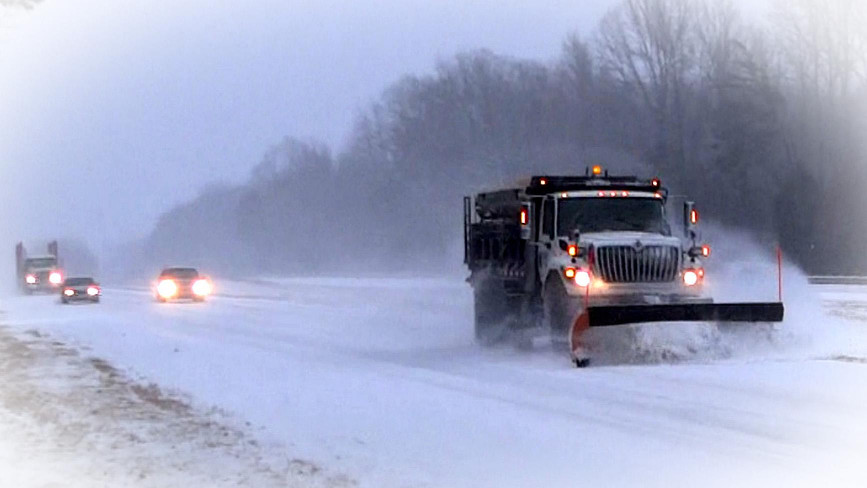
\includegraphics[width=\linewidth]{snowplow.jpg}
%% \end{columns}

%% \vspace{0.25 cm}
%% \begin{center}
%% \textcolor{blue}{\underline{\url{https://cms-big-data.github.io/}}}
%% \end{center}
%% \end{frame}

%% \begin{frame}{How to get the data into Spark}
%% \vspace{0.5 cm}
%% \small

%% \underline{\large \bf A year of trial-and-error in one slide}
%% \begin{center}
%% \begin{minipage}{0.8\linewidth}
%% \begin{enumerate}
%% \item \textcolor{darkblue}{Java Native Interface (JNI)} \\ No! This ought to be the right solution, but Java \\ and ROOT are both large, complex applications \\ with their own memory management: couldn't keep \\ them from interfering (segmentation faults).

%% \vspace{-2.2 cm}
%% \hfill 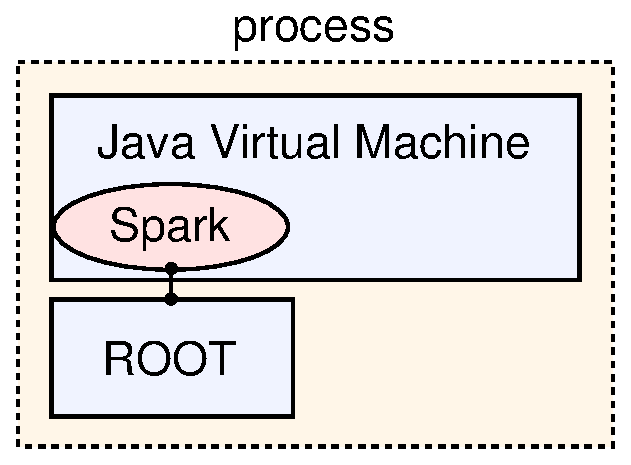
\includegraphics[height=1.65 cm]{root-spark.pdf}

%% \vspace{0.5 cm}
%% \item \textcolor{darkblue}{\normalsize Python as glue: PyROOT and PySpark in the same process}

%% \hfill 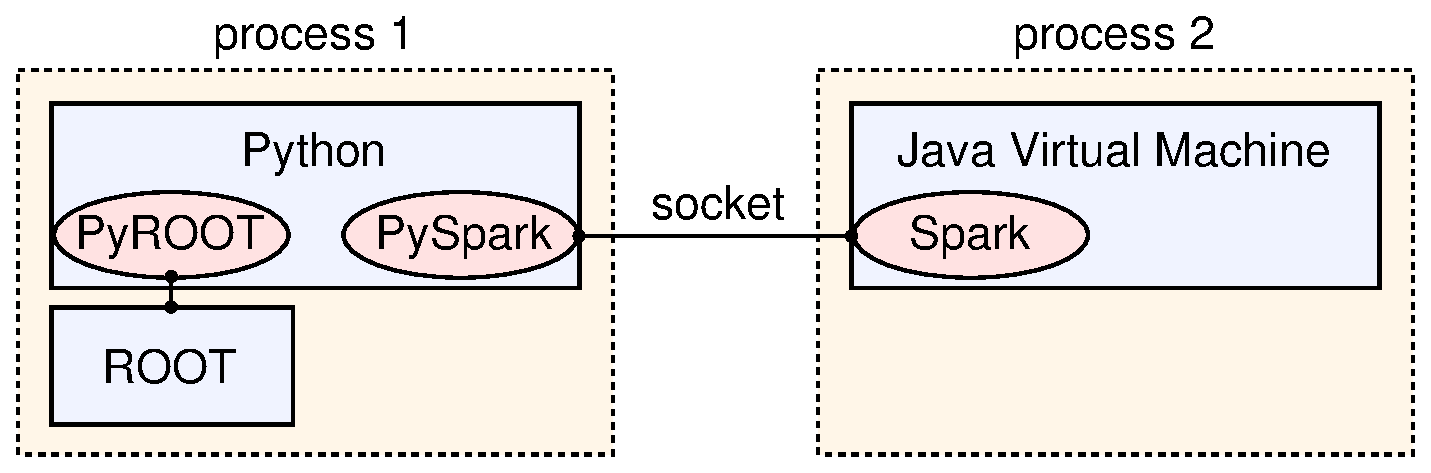
\includegraphics[height=1.65 cm]{pyroot-pyspark.pdf}

%% \vspace{-1.8 cm}
%% PySpark is a low-performance \\ solution: all data must be passed \\ over a text-based socket and \\ interpreted by Python.

%% \item \textcolor{darkblue}{\normalsize Convert to a Spark-friendly format, like Apache Avro}

%% We used this for a year. Efficient after conversion, but conversion step is awkward. Avro's C library is difficult to deploy.
%% \end{enumerate}
%% \end{minipage}
%% \end{center}

%% \begin{uncoverenv}<2->
%% \vspace{-5.2 cm}
%% \begin{center}
%% \fcolorbox{violet}{white}{\begin{minipage}{0.9\linewidth}
%% \vspace{0.5 cm}
%% \begin{center}
%% \begin{minipage}{0.9\linewidth}
%% \centering \large \textcolor{violet}{\bf These issues are historical. Industry-standard formats like Avro and Parquet can store complex physics events; we just happen to have a lot of data in ROOT files.}
%% \end{minipage}
%% \end{center}
%% \vspace{0.1 cm}
%% \end{minipage}}
%% \end{center}
%% \vspace{5 cm}
%% \end{uncoverenv}
%% \end{frame}

%% \begin{frame}{This was a missed opportunity for exporting physics solutions!}
%% \vspace{0.5 cm}
%% \large \textcolor{violet}{\bf ROOT was storing nested data structures in a columnar format (for faster access) over a decade before it was reinvented at Google.}

%% \vspace{-0.3 cm}
%% \begin{center}
%% \begin{minipage}{0.8\linewidth}
%% \vspace{0.5 cm}
%% \small Sergey Melnik, Andrey Gubarev, Jing Jing Long, Geoffrey Romer, Shiva Shivakumar, Matt Tolton, Theo Vassilakis. \textcolor{darkblue}{\normalsize {\it Dremel: Interactive Analysis of Web-Scale Datasets} (2010).}

%% \vspace{0.25 cm}
%% \fbox{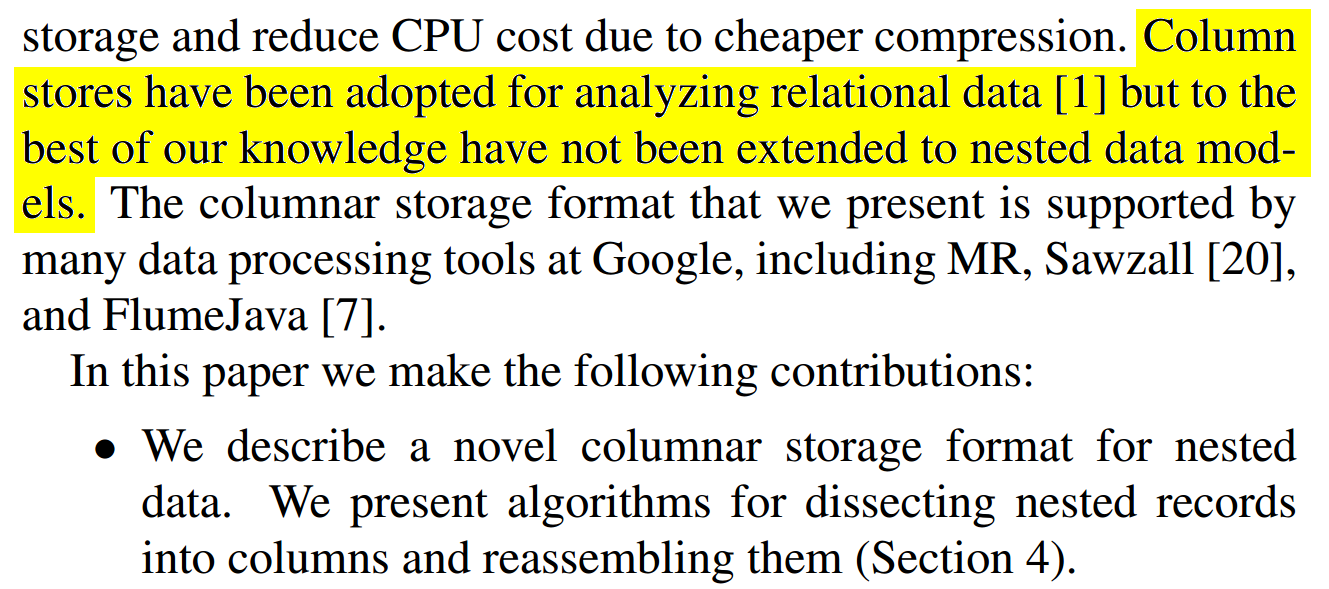
\includegraphics[width=\linewidth]{dremel-paper.png}}
%% \end{minipage}
%% \end{center}
%% \end{frame}

%% \begin{frame}{Easiest solution: reimplement ROOT I/O in Java}
%% \vspace{0.25 cm}
%% \begin{columns}
%% \column{1.1\linewidth}

%% \renewcommand{\arraystretch}{2.5}
%% \begin{tabular}{p{2 cm} c p{4.6 cm} p{5.25 cm}}
%% \centering root4j/ spark-root & Java/Scala & For Spark and other Big Data projects that run on Java. & Started by Tony Johnson in 2001, updated by Viktor Khristenko. \\
%% \centering \only<2->{JsRoot} & \only<2->{Javascript} & \only<1>{\mbox{\hspace{4 cm}} \mbox{\hspace{4 cm}}}\only<2->{For interacting with ROOT in the browser or standalone.} & \only<2->{Sergey Linev} \\
%% \centering \only<3->{rootio} & \only<3->{Go} & \only<3->{go-hep ecosystem in Go.} & \only<3->{Sebastien Binet} \\
%% \centering \only<4->{uproot} & \only<4->{Python} & \only<1-3>{\mbox{\hspace{4 cm}} \mbox{\hspace{4 cm}} \mbox{\hspace{4 cm}}}\only<4->{For quickly getting ROOT data into Numpy and Pandas for machine learning.}\vspace{-0.25 cm} & \only<4->{Jim Pivarski (me)} \\
%%  & \only<5->{Rust?} & & \\
%% \end{tabular}

%% \vspace{-6.25 cm}
%% \only<1>{{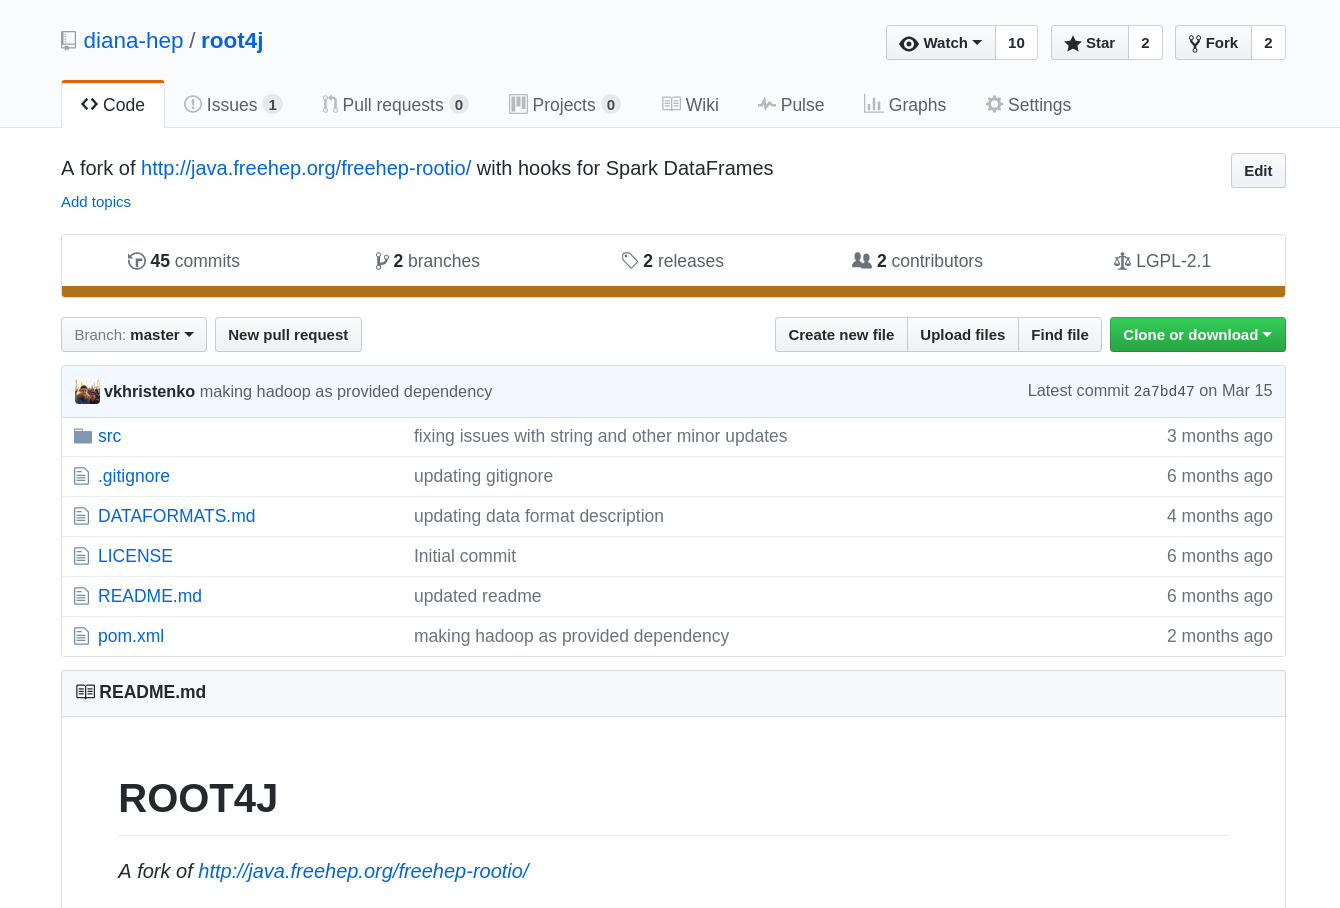
\includegraphics[width=\linewidth]{root4j.png}}}
%% \vspace{6 cm}
%% \end{columns}
%% \end{frame}

%% \begin{frame}[fragile]{Example session (\only<1>{native Spark, which is Scala}\only<2>{PySpark in Python})}
%% \vspace{0.35 cm}
%% \begin{center}
%% \begin{minipage}{0.9\linewidth}
%% Launch Spark with packages from Maven Central.
%% \small
%% \begin{onlyenv}<1>
%% \begin{minted}{bash}
%% spark-shell --packages org.diana-hep:spark-root_2.11:x.y.z, \
%%                        org.diana-hep:histogrammar_2.11:1.0.4
%% \end{minted}
%% \end{onlyenv}
%% \begin{onlyenv}<2>
%% \begin{minted}{bash}
%% pyspark     --packages org.diana-hep:spark-root_2.11:x.y.z, \
%%                        org.diana-hep:histogrammar_2.11:1.0.4
%% \end{minted}
%% \end{onlyenv}

%% \normalsize
%% Read ROOT files like any other DataFrame input source.

%% \small
%% \begin{onlyenv}<1>
%% \begin{minted}{scala}
%% val df = spark.sqlContext.read.root(
%%                           "hdfs://path/to/files/*.root")
%% \end{minted}
%% \end{onlyenv}
%% \begin{onlyenv}<2>
%% \begin{minted}{python}
%% df = sqlContext.read.format("org.dianahep.sparkroot") \
%%                     .load("hdfs://path/to/files/*.root")
%% \end{minted}
%% \end{onlyenv}

%% \vspace{-0.5 cm}
%% \small
%% \begin{verbatim}
%% df.printSchema()
%% root
%%  |-- met: float (nullable = false)
%%  |-- muons: array (nullable = false)
%%  |    |-- element: struct (containsNull = false)
%%  |    |    |-- pt: float (nullable = false)
%%  |    |    |-- eta: float (nullable = false)
%%  |    |    |-- phi: float (nullable = false)
%%  |-- jets: array (nullable = false)
%% \end{verbatim}
%% \end{minipage}
%% \end{center}
%% \end{frame}

%% \begin{frame}[fragile]{Example session (native Spark and PySpark)}
%% \vspace{0.35 cm}
%% \begin{center}
%% \begin{minipage}{0.9\linewidth}
%% \small
%% \begin{verbatim}
%% df.show()
%% +---------+--------------------+--------------------+
%% |      met|               muons|                jets|
%% +---------+--------------------+--------------------+
%% | 55.59374|[[28.07075,-1.331...|[[194.19714,-2.65...|
%% |39.440292|                  []|[[93.64958,-0.273...|
%% |2.1817229|[[5.523367,-0.375...|[[96.09923,0.7058...|
%% |  80.5822|[[48.910114,-0.17...|[[165.2686,0.2623...|
%% | 84.43806|                  []|[[51.87823,1.6442...|
%% | 84.63146|[[33.84279,-0.062...|[[137.74776,-0.45...|
%% | 393.8167|[[25.402626,-0.66...|[[481.8268,-1.115...|
%% |  75.0873|                  []|[[144.62373,-2.21...|
%% |2.6512942|[[6.851382,2.3145...|[[72.08256,-1.713...|
%% |36.753353|                  []|[[72.7172,-1.3265...|
%% +---------+--------------------+--------------------+
%% only showing top 10 rows
%% \end{verbatim}
%% \end{minipage}
%% \end{center}
%% \end{frame}

%% \begin{frame}[fragile]{Example session (\only<1>{Spark}\only<2>{PySpark})}
%% \vspace{0.1 cm}
%% \small
%% \begin{onlyenv}<1>
%% \begin{minted}{scala}
%% // Bring dollar-sign notation into scope.
%% import spark.sqlContext.implicits._


%% // Compute event weight with columns and constants.
%% df.select(($"lumi"*xsec/nGen) * $"LHE_weight"(309)).show()

%% // Pre-defined function (notation's a little weird).
%% val isGoodEvent = (
%%     ($"evtHasGoodVtx" === 1) &&
%%     ($"evtHasTrg" === 1)     &&
%%     ($"tkmet" >= 25.0)       &&
%%     ($"Mu_pt" >= 30.0)       &&
%%     ($"W_mt" >= 30.0))

%% // Use it.
%% println("%d events pass".format(
%%                     df.where(isGoodEvent).count()))
%% \end{minted}
%% \end{onlyenv}\begin{onlyenv}<2>
%% \begin{minted}{python}
%% # Python trick: make columns Python variables.
%% for name in df.schema.names:
%%     exec("{0} = df['{0}']".format(name))

%% # Look at a few event weights.
%% df.select((lumi*xsec/nGen) * LHE_weight[309]).show()

%% # Pre-defined function (notation's a little different).
%% isGoodEvent = (
%%     (evtHasGoodVtx == 1) &
%%     (evtHasTrg == 1)     &
%%     (tkmet >= 25.0)      &
%%     (Mu_pt >= 30.0)      &
%%     (W_mt >= 30.0))

%% # Use it.
%% print "{} events pass".format(
%%                   df.where(isGoodEvent).count())
%% \end{minted}
%% \end{onlyenv}
%% \end{frame}

%% \begin{frame}[fragile]{Example session (\only<1>{Spark}\only<2->{PySpark})}
%% \vspace{0.1 cm}
%% \small
%% \begin{onlyenv}<1>
%% \begin{minted}{scala}
%% // Use Histogrammar to make histograms.
%% import org.dianahep.histogrammar._
%% import org.dianahep.histogrammar.sparksql._
%% import org.dianahep.histogrammar.bokeh._

%% // Define histogram functions with SparkSQL Columns.
%% val h = df.Label(
%%          "muon pt" -> Bin(100, 0.0, 50.0, $"Mu_pt"),
%%          "W mt" -> Bin(100, 0.0, 120.0, $"W_mt"))

%% // Plot the histograms with Bokeh.
%% val bokehhist = h.get("muon pt").bokeh()
%% plot(bokehhist)
%% val bokehhist2 = h.get("W mt").bokeh()
%% plot(bokehhist2)
%% \end{minted}
%% \end{onlyenv}\begin{onlyenv}<2->
%% \begin{minted}{python}
%% # Use Histogrammar to make histograms.
%% from histogrammar import *
%% import histogrammar.sparksql
%% histogrammar.sparksql.addMethods(df)

%% # Define histogram functions with SparkSQL Columns.
%% h = df.Label(
%%       muon_pt = Bin(100, 0.0, 50.0, Mu_pt),
%%       W_mt = Bin(100, 0.0, 120.0, W_mt))

%% # Plot the histograms with PyROOT.
%% roothist = h.get("muon_pt").plot.root("muon pt")
%% roothist.Draw()
%% roothist2 = h.get("W_mt").plot.root("W mt")
%% roothist2.Draw()
%% \end{minted}
%% \end{onlyenv}

%% \vspace{-2.7 cm}
%% \begin{uncoverenv}<3>
%% \mbox{ } \hfill 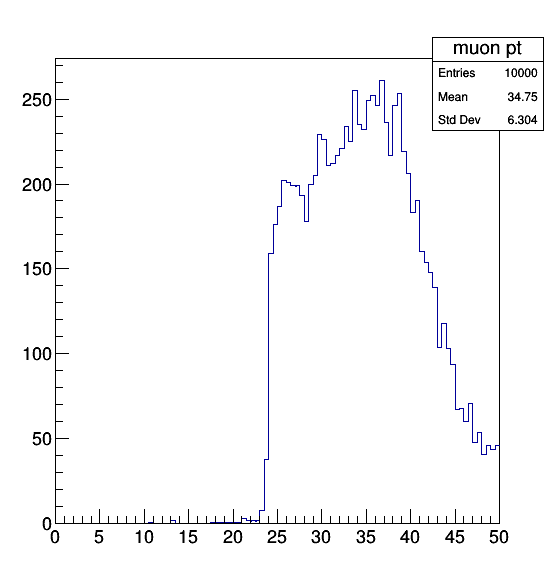
\includegraphics[width=3.8 cm]{muonpt.png}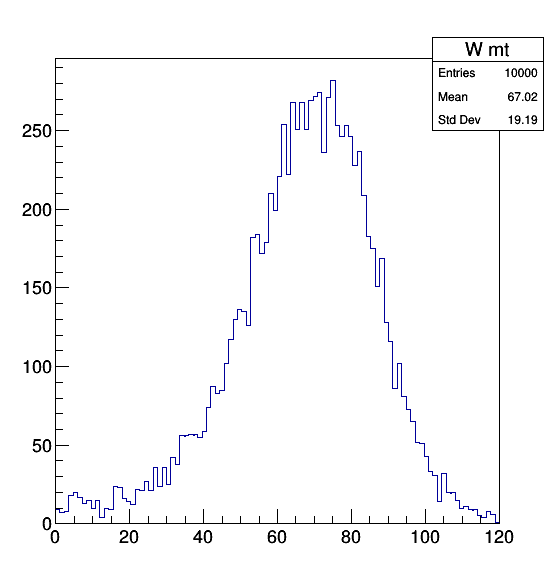
\includegraphics[width=3.8 cm]{wmt.png}
%% \end{uncoverenv}
%% \end{frame}

\begin{frame}{}

\end{frame}


\end{document}

%% \begin{frame}{Conclusions slide?}
%% \vspace{0.5 cm}
%% \begin{center}
%% \hspace{1 cm}\only<1>{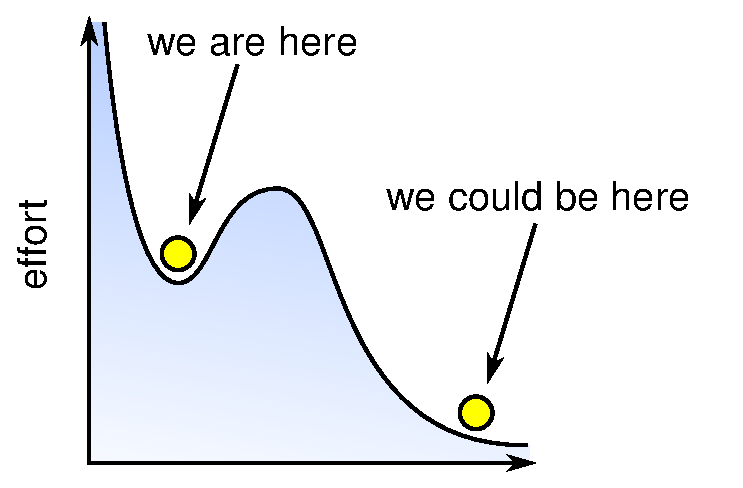
\includegraphics[width=0.65\linewidth]{effort0.pdf}}\only<2>{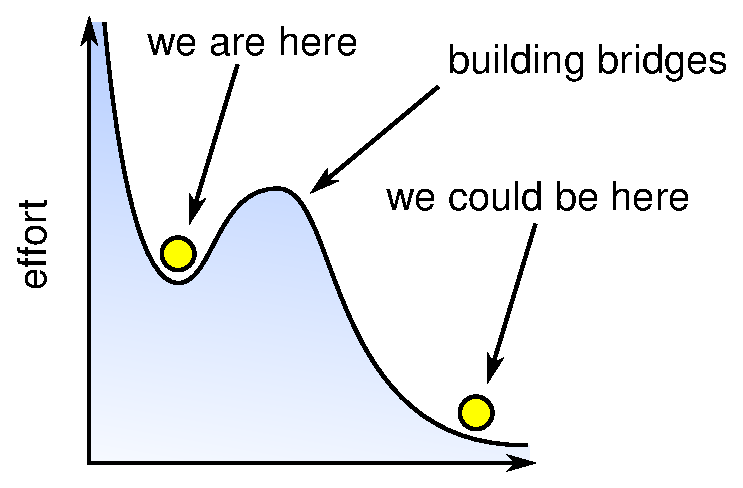
\includegraphics[width=0.65\linewidth]{effort.pdf}}
%% \end{center}
%% \end{frame}
